\chapter{Algorithmes utilisés}
    La recherche des algorithmes et leur développement fut l'un des gros morceaux du projet. Cette partie pris une semaine de développement.

    \section{Design pattern: Lexer/Parser}
        \begin{figure}[h]
            \begin{center}
                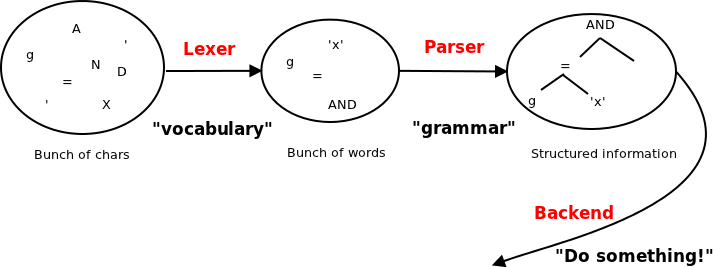
\includegraphics[scale=0.5]{lexer_parser.png}
            \end{center}

            \caption{Représentation du Lexer/Parser}
            \label{Représentation du Lexer/Parser}
        \end{figure}

        \paragraph{}
            Le choix a été fait de remplir un des objectifs secondaires du cahier des charges, ``l'imbrication libre des instructions''.
            \\ Le problème a été traité de manière traditionnelle, une utilisant le design pattern lexer/Parser.
            \\ Le lexer, est ``l'analyseur lexical''. Il transforme une série de caractères en ``tokens'', qui sont des chaînes de caractères définies au préalable.
            \\ Ainsi, un mot est un token ``T\_STRING'', un chiffre est un token ``T\_SCALAR'' ou encore une matrice un ``T\_MATRIX''. Au niveau du code, ces tokens sont représentés par des objets (voir \ref{lib/token.h}) ayant chacun la valeur de la chaine de caractère reconnue associée à leur type. Exemple : le chiffre 3 est un objet Token de type ``T\_SCALAR'' et de valeur ``3''.
            \\ La reconnaissance de ces tokens se fait par regex successive sur la chaine de caractère ce que l'une d'entre elle fonctionne.
      
            \begin{figure}[h]
                \begin{center}
                    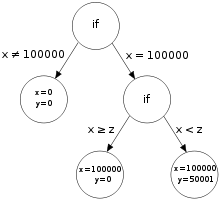
\includegraphics[scale=1]{syntax_tree.png}
                \end{center}

                \caption{Création d'un arbre d'execution. Des noeuds conditionnels sont représentés}
                \label{Représentation arbre syntaxique}
            \end{figure}

        \newpage

        \paragraph{}
            Une fois l'expression analysée, il faut l'exécuter. Le parser passe en revue tous les tokens en essayant de reconnaître des ``motifs'' d'expression cohérentes. Il les assemble ensuite en Node (voir \ref{lib/node.h}), qui sont comme leur nom l'indique des noeuds d'expression. Un exemple de noeud est le noeud d'assignation, ayant comme motif un nom de variable et une expression séparée par un signe égal.


            Le code est pensé de manière modulaire, il est ainsi possible de rajouter d'autres types de noeud comme des noeuds conditionnels par exemple, et ainsi étendre l'analyseur d'expression en un véritable interpréteur de language.
            \\ Les Nodes créées, elles sont ensuite assemblées en arbre et ensuite exécutée. Nous allons maintenant voir par quelle méthode les  expressions sont interprétées.

    \section{Execution des expression: Notation Polonaise Inversée}
        L'execution des expressions peut se faire de plusieurs manières. La première qui a été abordée puis abandonnée par la suite, est la création d'un arbre syntaxique similaire à l'arbre d'éxecution introduit à la section précédente. Le problème avec cette manière de fonctionner est qu'elle est bien plus lourde niveau code et donc source de bugs. Une implémentation de cette méthode a néammoins été produite et reste visible dans l'historique des commits du projet.
        \\ L'autre manière d'aborder le problème et qui a été retenue pour le projet est la conversion de l'expression sous sa forme infixe (forme usuelle, utilisant les parenthèses) en notation polonaise inversée, une forme d'expression bien plus simple a exécuter qui ne comprend ni parenthèses ni priorité d'opérateurs.
        \\ Voici un exemple simple d'expression.
        \begin{equation}
            (2 + 4) * 2
        \end{equation}
        Une fois convertis en notation polonaise inversée, celà donne l'expression suivante.
        \begin{equation}
            2 4 + 2 *
        \end{equation}
        Le principe est d'empiler opérandes et opérateurs, chaque opérateurs opérant sur les deux opérandes qui le précède.
        \\ Cette méthode, très connue et largement utilisée par les compilateurs nous a permis de trouver une implémentation de l'algorithme permettant la conversion de l'expression, et quant à l'éxecution de l'expression, c'est un jeux d'enfant.